
\documentclass[xcolor=x11names,9pt]{beamer}

%%
%% PACKAGES
%%

\usepackage{algorithmic}
\usepackage{graphicx}
\usepackage{microtype}
\usepackage{pgf}
\usepackage{tikz}
\usetikzlibrary{decorations.fractals}
\usetikzlibrary{arrows,automata,positioning}
\usepackage[normalem]{ulem}


%%
%% BEAMER LAYOUT ETC
%%

\geometry{paperwidth=140mm,paperheight=105mm}
\usetheme{Antibes}
\setbeamertemplate{blocks}[rounded][shadow=false]
 
%% gets rid of bottom navigation bars
%% gets rid of navigation symbols
\setbeamertemplate{footline}[frame number]{}
\setbeamertemplate{navigation symbols}{}


\setbeamerfont{block title}{size=\small}
\setbeamerfont{block body}{size=\small}
\setbeamerfont{frametitle}{size=\large}
\setbeamersize{text margin left=1em,text margin right=1em}


%% uncomment following for top navigation bar
\setbeamertemplate{headline}{}
% \useoutertheme[subsection=false,shadow]{miniframes}
%% hack to put circles next to sections
%\usepackage{etoolbox}
%\makeatletter
%\patchcmd{\slideentry}{\advance\beamer@tempdim by -.05cm}{\advance\beamer@tempdim by\beamer@vboxoffset\advance\beamer@tempdim by\beamer@boxsize\advance\beamer@tempdim by 1.2\pgflinewidth}{}{}
%\patchcmd{\slideentry}{\kern\beamer@tempdim}{\advance\beamer@tempdim by 2pt\advance\beamer@tempdim by\wd\beamer@sectionbox\kern\beamer@tempdim}{}{}
%\makeatother
%\setbeamercolor*{lower separation line head}{bg=Red4} 

% rectangles for bullets
\useinnertheme{default}
\usefonttheme{serif}
\usepackage{palatino}

\setbeamerfont{title like}{shape=\scshape}
\setbeamerfont{frametitle}{shape=\scshape}

\setbeamercolor*{normal text}{fg=black,bg=white}  
\setbeamercolor*{alerted text}{fg=Red4} 
\setbeamercolor*{example text}{fg=black} 
\setbeamercolor*{structure}{fg=black} 
 
\setbeamercolor*{palette tertiary}{fg=black,bg=black!10} 
\setbeamercolor*{palette quaternary}{fg=black,bg=black!10} 


%%
%% NOTATION
%% 

\newcommand*\varhrulefill[1][0.4pt]{\leavevmode\leaders\hrule height#1\hfill\kern0pt}
\newcommand{\x}[1]{\boldsymbol#1}
\newcommand{\z}[1]{\mathcal{#1}}
%\newcommand{\w}[1]{\mathscr{#1}}
\newcommand{\w}[1]{\texttt{#1}}
 

\begin{document}

%%
%% FRAMES
%%

\section{\scshape Introduction}
\begin{frame}
 
 	\title{Exact and heuristic methods for trading-off makespan and stability in stochastic project scheduling}
 	\subtitle{\textsc{MISTA 2015}}
	\author{
		K.S. Mountakis, \and T. Klos, \and C. Witteveen, \and B. Huisman  
	}
	\date{
 		\includegraphics[width=0.25\textwidth]{tu_logo_wide}
		\\
	} 
	\titlepage
	
\end{frame}

\begin{frame}{Motivation \& Preliminaries}
\only<1,2>{
	Project scheduling literature: mostly RCPSP
	\begin{itemize}
		\item activities, resources, precedence and resource constraints
	 	\item durations = single-point estimates
	  	\item NP-Hard (Blazewicz et al. 1983)
	\end{itemize}
	
	\bigskip
	 
	\onslide<2>{How useful for real-world projects?}
}

\only<3>{
	Example RCPSP \& solution
	\medskip
	
 	\centering{\includegraphics[width=0.7\textwidth]{fig-s1b}}
}
\end{frame}


\begin{frame}{Motivation \& Preliminaries}

\onslide<1->{
\textbf{Reactive} stochastic project scheduling: S-RCPSP
\begin{itemize}
 	\item stochastic durations $\x{D}=(D_1, \ldots, D_n)$ with known $\mathbb{P}[D_i = t]$
 	\item solution = \sout{fixed schedule} scheduling policy $\Pi$
  	\item find $\Pi$ that minimizes $\mathbb{E}[\max_{i=1,\ldots,n} (S_i(\Pi,\x{D}) + D_i)]$
  	\item RCPSP generalization (at least as hard)
\end{itemize}

\medskip
}

\onslide<2->{
	Various classes of $\Pi$
 	\begin{itemize}
		\item list-based policies,  earliest-start policies, etc.  (M{\"o}hring et al. 1984,1985)
		\item exact procedures (Stork 2000)
		\item meta-heuristics (e.g. Ballest{\'\i}n 2007, Ashtiani et al. (2011))
	\end{itemize}
}

\end{frame}

\begin{frame}{Motivation \& Preliminaries}

Example S-RCPSP \& solution
\medskip
\begin{center}\includegraphics[width=0.7\textwidth]{fig-s1c}\end{center}
 
\onslide<2->{
	\medskip
	Disadvantage: no fixed-time schedule at all
}

\end{frame}


\begin{frame}{Motivation \& Preliminaries}

\only<1,2>{
	\textbf{Proactive-reactive} stochastic project scheduling
	\begin{itemize}
	 	\item stochastic durations $\x{D}=(D_1, \ldots, D_n)$ with known $\mathbb{P}[D_i = t]$
	 	\item solution = (proactive schedule $\x{t}$, reactive policy $\Pi$)
	 	\begin{itemize}
	 		\item $\x{t}=(t_1,\ldots,t_n)$: buffered and can more-or-less be trusted   
	  		\item $\Pi$: what to do in case of buffer overruns
	  	\end{itemize}
	  	\item \textbf{railway mode}: $S_i(\Pi, \x{t}) \geq t_i$
	  	\item find $(\x{t},\Pi)$ that balances \emph{expected instability} and \emph{expected makespan}
	\end{itemize}
	
	\bigskip
	\onslide<2>{
		Minimize both
		\begin{enumerate}
		\item expected instability
		\[
			\mathbb{E}[\sum_{i} (S_i((\Pi,\x{t}),\x{D}) - t_i)]
		\]
		
		\item expected makespan
		\[
			\mathbb{E}[\max_{i} (S_i((\Pi,\x{t}),\x{D}) + D_i)]
		\]
		\end{enumerate}
	}
}

\only<3>{
	Tuning some tradeoff parameter
	\bigskip
	\begin{center}\includegraphics[width=0.7\textwidth]{fig-tradeoff}\end{center}
}

\end{frame}


\begin{frame}{Our Approach}
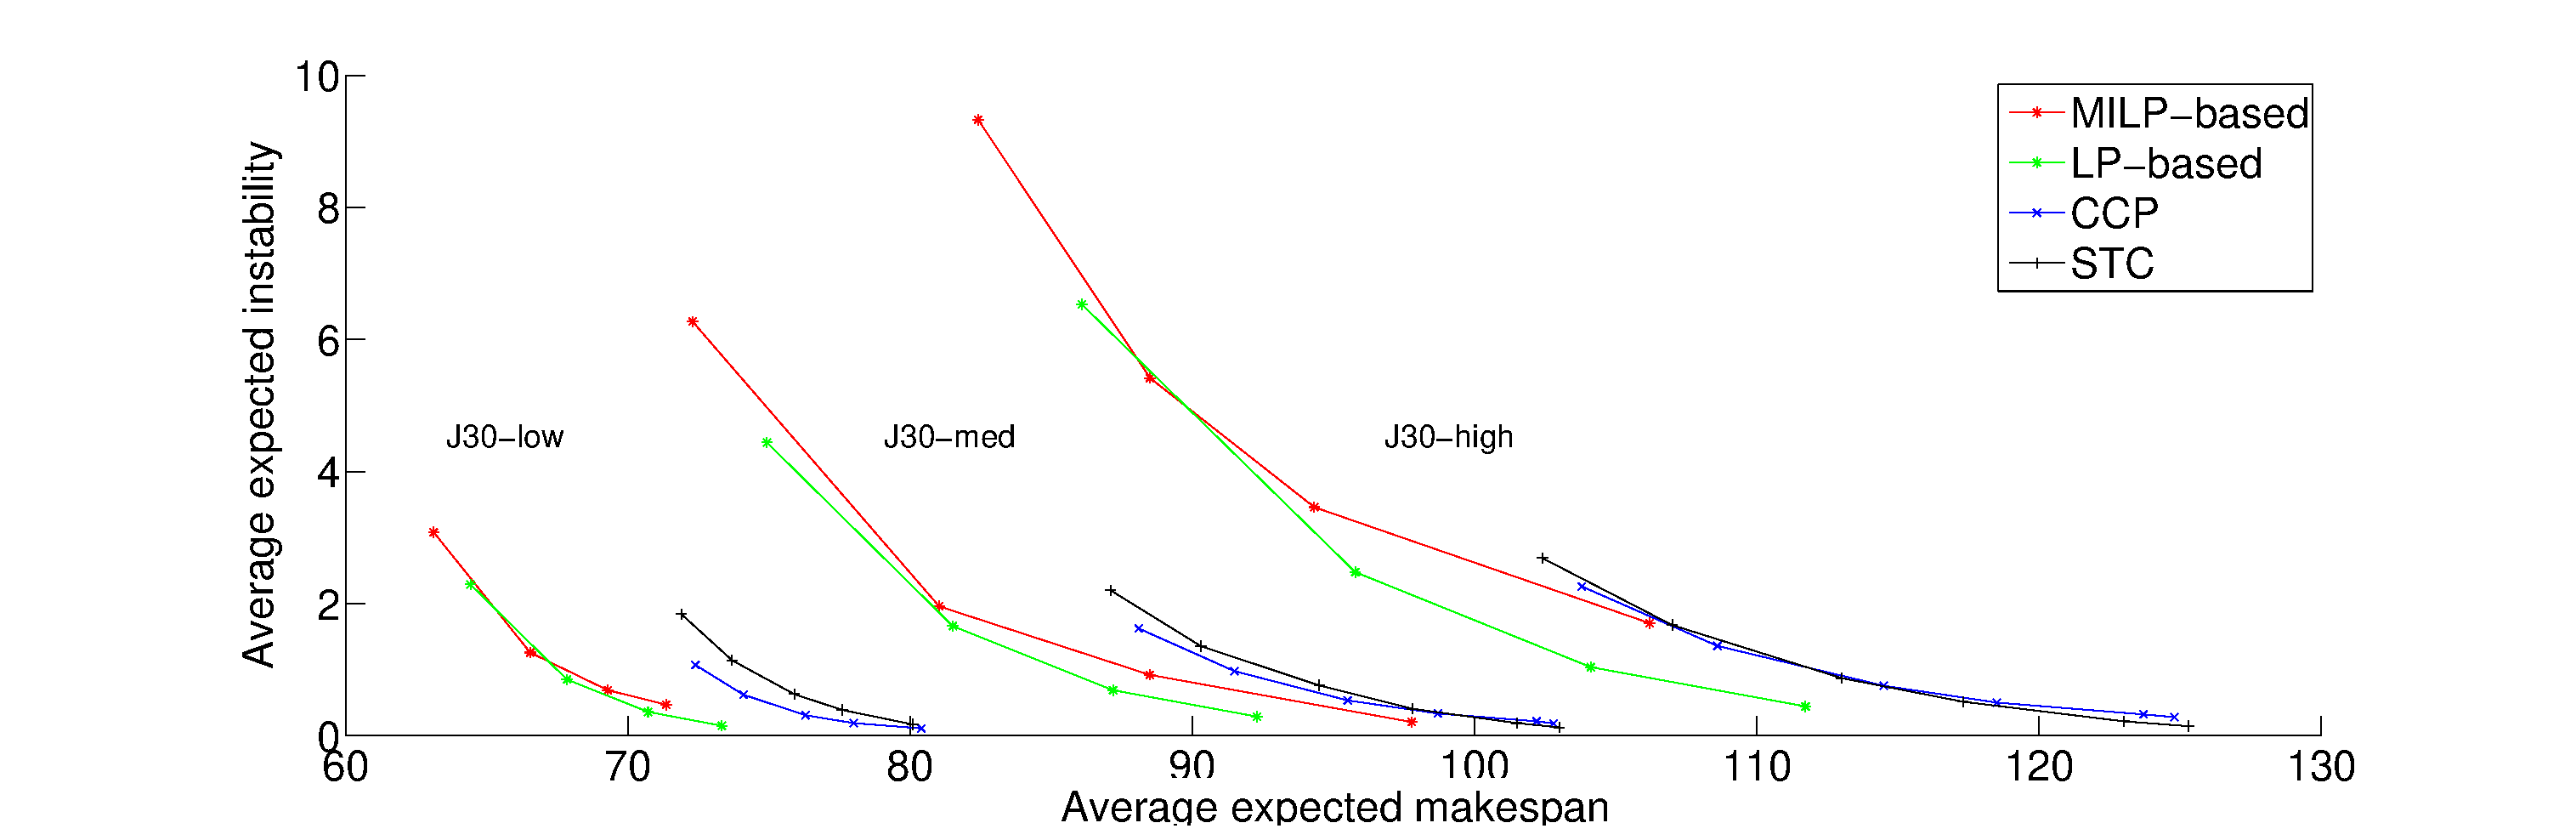
\includegraphics[width=1.05\textwidth]{../figure1.eps}
\medskip
\begin{itemize}
	\item \color{blue}CCP model (Lamas and Demeulemeester, Journal of Scheduling, 2015)\color{black}
	\item STC heuristic (Van de Vonder et al., EJOR, 2008)
	\item \color{red}MILP-based heuristic \color{black} ($\z{O}(2^m)$ with $m < n$)
	\item \color{green}LP-based heuristic \color{black} ($\z{O}(n^4)$)
\end{itemize}
\end{frame}


\begin{frame}{Our Approach} 
Define the Proactive Stochastic (PS-)RCPSP
\begin{itemize}
	\item focus specifically on earliest-start (es-)policies
	\item find $(\z{E}, \x{t})$ together as a pair
	\item to minimize $\alpha \cdot \texttt{Exp.Makespan}(\z{E},\x{t}) + (1-\alpha) \texttt{Exp.Instability}(\z{E},\x{t})$
\end{itemize}

\medskip

\begin{center}
	\includegraphics[width=0.6\textwidth]{fig-sol2}
\end{center}

\medskip
Stochastic optimization problem

\end{frame}


\begin{frame}{Our Approach: Solving PS-RCPSP}

\begin{center}
\only<1>{\includegraphics[height=0.8\textheight]{methods1}}
\only<2>{\includegraphics[height=0.8\textheight]{methods2}}
\only<3>{\includegraphics[height=0.8\textheight]{methods3}}
\end{center}

\end{frame}


\begin{frame}{Thank you; Questions?}

\begin{center}
\includegraphics[height=0.8\textheight]{methods3}
\end{center}

\end{frame}

   

\end{document}
